\section{Introduction}
\label{sec:intro}
\acp{ICD} are life-saving medical devices.
An \ac{ICD} is implanted under the shoulder, and connects directly to the heart muscle though two electrodes and continuously measures the heart's rhythm (Fig. \ref{fig:icd}).
If it detects a potentially fatal accelerated rhythm, the \ac{ICD} delivers a high-energy electric shock or sequence of pulses through the electrodes to reset the heart's electrical activity.
Without this therapy, this \emph{tachycardia} is usually fatal within seconds of onset.
In the US alone, 10,000 people receive an \ac{ICD} every month.
Studies have presented evidence that patients implanted with \acp{ICD} have a mortality rate reduced by up to 31\% \cite{maditrit}.

Unfortunately, \acp{ICD} suffer from a high rate of \emph{inappropriate therapy} due to poor detection of the current rhythm on the part of the \ac{ICD}.
Inappropriate shocks increase patient stress, reduce their quality of life, and are linked to increased morbidity \cite{shock_mortality}.
Depending on the particular ICD and its settings, the rates of inappropriate therapy range from 46\% to 62\% of all delivered therapy episodes \cite{GoldABBTB11_RIGHTresults}.
Current practice for \ac{ICD} verification relies heavily on testing and software cycle reviews.
With the advent of computer models of the human heart, \emph{Model-Based Design} (MBD) can and should play a prominent role in \ac{ICD} development.
This paper presents hybrid system models of the human heart and of the common modules of \acp{ICD} currently on the market, and shows that the closed loop formed by these models is \emph{formally verifiable}.
The objective is to develop model checkers for \acp{ICD} to further their MBD process.
\begin{figure}[t]
	\centering
	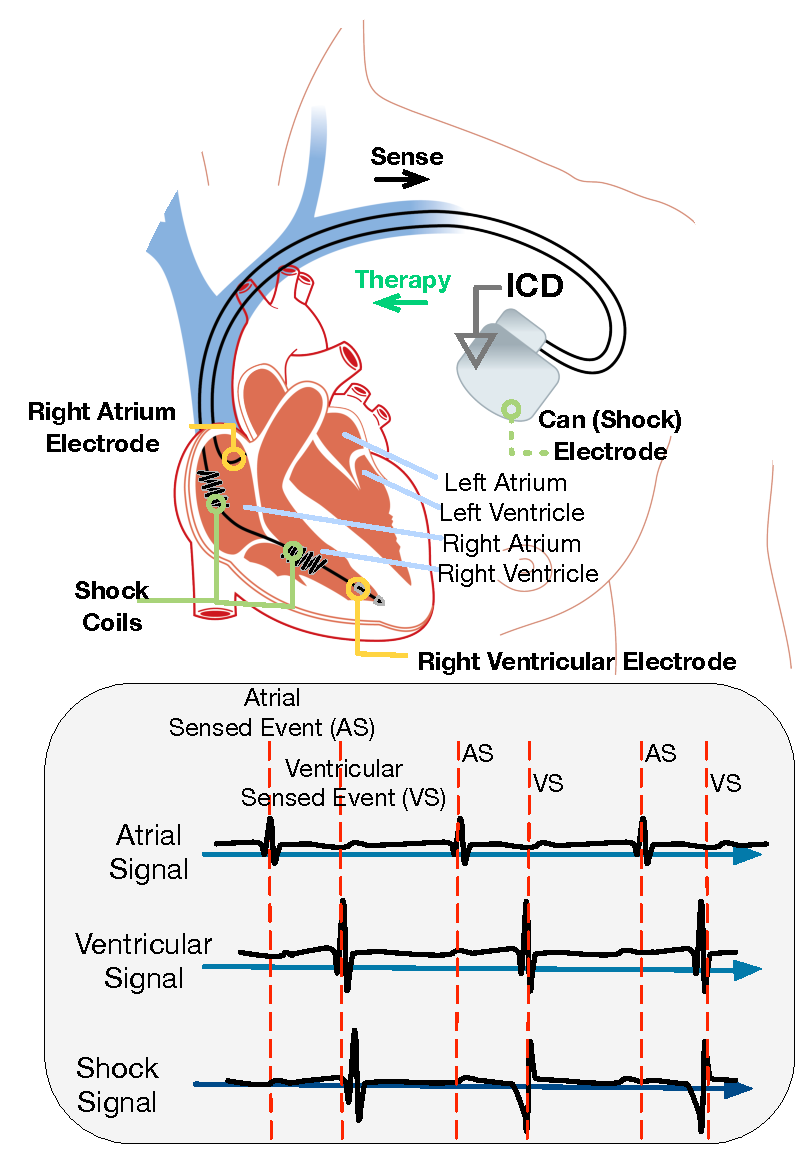
\includegraphics[scale=0.3]{figures/figICD}
	\vspace{-10pt}
	\caption{\small ICD connected to a human heart via two electrodes. The ICD monitors three electrical signals (known as electrograms) traversing the heart muscle.}
	\label{fig:icd}
	\vspace{-10pt}
\end{figure}

\begin{figure*}[t]
	\centering
	\vspace{-10pt}
	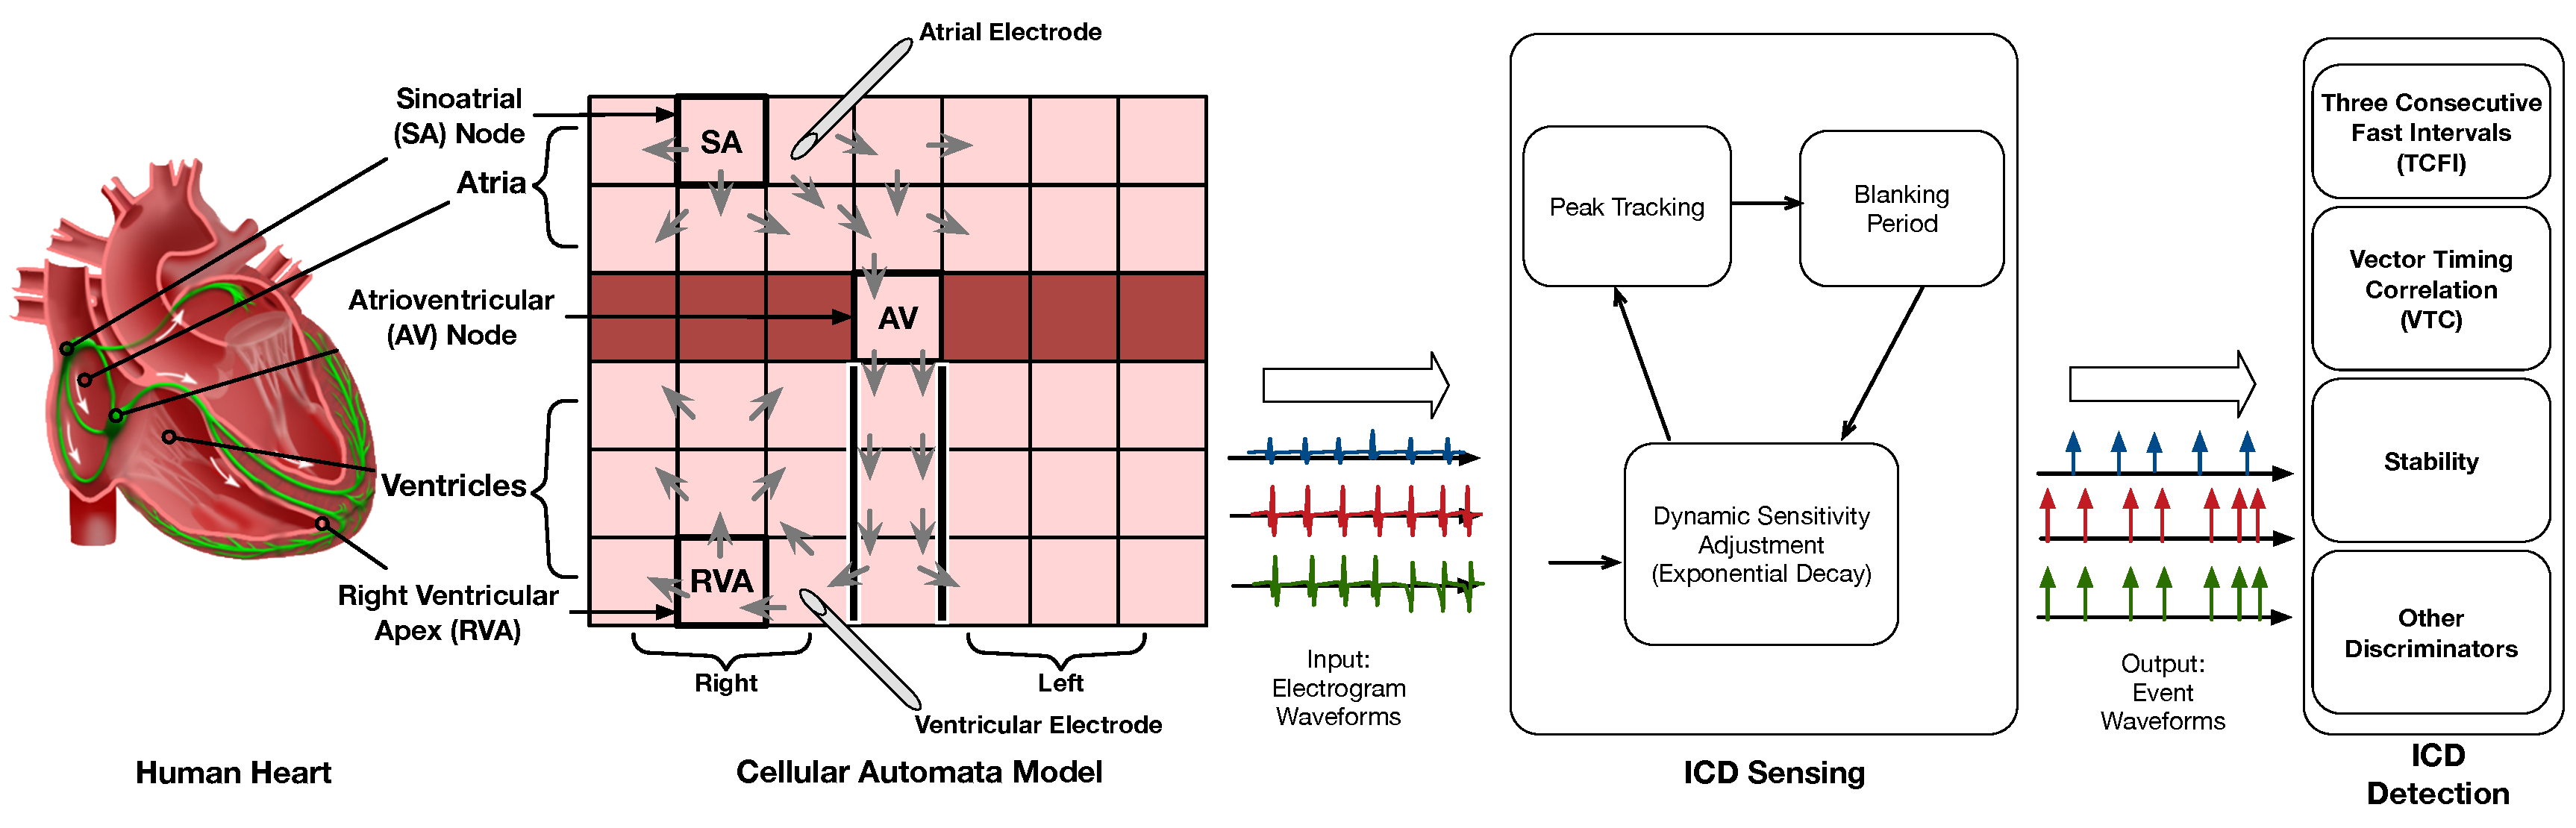
\includegraphics[scale=0.28]{figures/overviewFigure}
	\vspace{-10pt}
	\caption{\small The whole heart is modeled as a 2D mesh of cells (Section \ref{sec:heartcellularautomata}). The \ac{ICD} electrodes are shown in the right atrium and ventricle. The electrogram signals measured through the electrodes are processed by the sensing module (ICD Sensing, see Section \ref{sec:sensing}). The detection algorithm (Section \ref{sec:discriminators}) determines the current rhythm using the processed signal (ICD Detection). \textbf{AV}: atrio-ventricular node, \textbf{RVA}: right ventricle apex, \textbf{SA}: sino-atrial node.}
	\label{fig:overview}
	\vspace{-10pt}
\end{figure*}
		%For Sensing ($\Sys_{Sense}$), states not shown in a mode have a 0 derivative, e.g., $\dot{eF}=0$ in all modes. $y(t) = |\egm(t)|$.}
Earlier work on verification of medical devices (formal or otherwise) focuses on pacemakers.
%Broadly speaking, this is a device that monitors the heart rate and increases it if it drops below some threshold.
In \cite{TACAS12} the authors developed timed automata models of both heart and pacemaker, which allows formal verification of LTL properties of the heart+pacemaker loop.
In \cite{Chen14_Quantitative} the authors perform probabilistic testing-based verification of Hybrid I/O automata models of heart and pacemaker.
However, they can not be symbolically verified.
Later work on pacemakers \cite{Mery} develops a formalized \ac{CA} model of the heart and uses Event-B for expressing its properties.
\ac{CA}-based models \cite{BartocciCBESG09_HIOAmodeling},\cite{Mery} are appealing due to their intuitive correspondence with the heart's anatomy and function and their relative computational simplicity.

%Because the pacemaker only reads the timing of events in the heart, a timed automata model of both heart and device are appropriate.
The \ac{ICD} algorithms are more complex than a pacemaker's: an \ac{ICD} measures the timing of events, but also measures and processes the \emph{morphology} of the electrical signal in the heart to distinguish many types of arrhythmias.
Thus, we need three models for \ac{ICD} verification: a timing and voltage model of the heart, a model of the \ac{ICD}'s algorithms, and a model for voltage measurement by the \ac{ICD} electrodes.
This takes the model out of the realm of timed automata and into hybrid automata proper.

The first contribution of this paper is to develop a hybrid system model of the heart, the \ac{ICD} measurement process, and of the algorithmic components of \acp{ICD} from most major manufacturers on the market.
We show that the composition of these three models can be \emph{formally verified}: specifically, it admits a finite bisimulation \cite{AlurHLP00ieee}.
The \ac{ICD} models presented here are the first formalization of \ac{ICD} operation to the best of our knowledge.

To establish this result we use the theory of STORMED hybrid systems \cite{VladimerouPVD08_STORMED}, a class of hybrid systems that have finite bisimulations.
Our second contribution is two general results for STORMED systems.
First we prove that parallel compositions of STORMED systems yield STORMED systems.
Secondly, we show that any (definable) over-approximate reach tubes can replace the exact flows of a STORMED system, yielding a system that still admits a finite simulation (but no longer a bisimulation). 
Finally, we show that the reach sets computed by the reachability tool SpaceEx \cite{FrehseCAV11} are definable and so can be used to build the simulation.
%This improves on the approach of \cite{PrabhakarVVD09_toklerant} which requires polynomial approximation of the flows, a process that is often manual or restricted to sub-classes of STORMED systems.
%Moreover it obviates the need to perform an expensive quantifier elimination step.


Our interest in not simply in a particular manufacturer's arrhythmia detection algorithm: rather, we are interested in those components that are common to most of them, thus making our results relevant to them.
The components we model or some variation on them are included in the \acp{ICD} of Boston Scientific, Medtronic, Saint-Jude Medical and Biotronik.
%It is promising that a sufficiently accurate and empirically validated heart model is still amenable to finite symbolic manipulation. 
%One of the crucial factors enabling this is the fact that \ac{ICD} operation is bounded-time, in the sense that there are natural reset points in the algorithm, at which the test may be considered to have ended.
This is the first example of a practical STORMED system that the authors are aware of.
In future work we will implement a model checker for this type of systems in order to verify interesting closed-loop properties of heart and \ac{ICD}.

\textbf{Organization}. 
Section \ref{sec:preliminaries} covers some preliminaries on hybrid systems.
Sections \ref{sec:heartcellularautomata} presents the heart model,
and Sections \ref{sec:sensing}-\ref{sec:discriminators} model the \ac{ICD}.
Sections \ref{sec:compositionality} and \ref{sec:simulationAprox} prove general results on STORMED systems that are used in the modeling: namely that a definable over-approximation of the flows such as that computed by SpaceEx preserves finiteness of the simulation, and that compositions of STORMED systems are STORMED.

Some material is relegated to an appendix, which is attached to the end of this paper for the reviewers' convenience. In the final version of this paper, the appendix will be moved online.


%\paragraph{Related work}
%
%[Bartocci et al " Modeling and simulation of cardiac tissue using hybrid I/O automata."] model the myocytes using HIOA for simulation purposes. Their model's semantics (the generated trajectories) are similar to ours (they add a "stimulated" mode, we add an "upstroke2" mode), but the objective is simulation and they don't show any model checking. Also there is no measurement model.
%
%[Kwiatowska's "Fomral modeling and verification of rate-adaptive pacemakers" ] deals with pacemakers only, and models the measurement only through binary events, and does not do model checking.
%
%[KWIATOWSKA "Estimation and verification of hybrid heart models for personalized medicine and wearable devices"] uses same TIOA model of heart cells and verifies probabilistic properties of pacemakers
%
%[Brihaye thesis] elaborated on o-minimal systems but not STORMED systems,
%
%kwiatowska parameter synthesis, 
%
%[Kwiatowska's Invariant Verification of Nonlinear Hybrid Automata Networks of Cardiac Cells,]
%
%
%Background: Pappas and girard's TAC09 paper
